\documentclass[12pt]{article}
\usepackage[utf8]{vietnam}
\usepackage{tikz}
\begin{document}
	\centerline{\Large\bfseries \textcolor{blue}{CÁCH NHÂN ĐA THỨC NGẮN GỌN}}
	\vspace*{5mm}
	\centerline{\bfseries Phạm Đăng Long}
	\centerline{\itshape Chuyên A0 - ĐHKHTN}
	\vspace*{1cm}
	{\noindent\bfseries Ví dụ:} Nhân $(3x^3+4x^2-5x+2)$ với $(2x^2+1)$.
	\begin{center}
		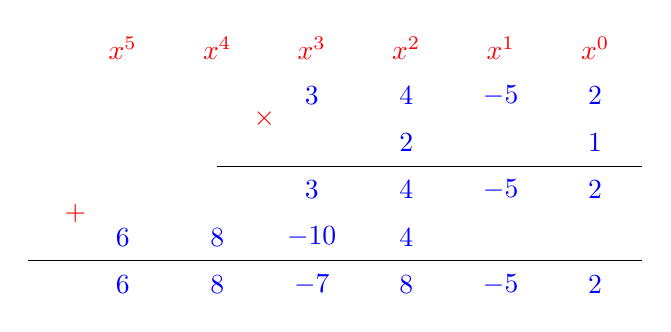
\begin{tikzpicture}[xscale=1.2,yscale=.6,blue]
			\foreach \i in {0,...,5}
			\path[red] (-\i,1) node{$x^{\i}$};
			\path
			(0,0) node{$2$}
			++(-1,0) node{$-5$}
			++(-1,0) node{$4$}
			++(-1,0) node{$3$}
			(-3.5,-.5) node[red]{$\times$}
			(0,-1) node{$1$} +(-2,0) node{$2$}
			(0,-2) node{$2$}
			++(-1,0) node{$-5$}
			++(-1,0) node{$4$}
			++(-1,0) node{$3$}
			(-5.5,-2.5) node[red]{$+$}
			(-2,-3) node{$4$}
			++(-1,0) node{$-10$}
			++(-1,0) node{$8$}
			++(-1,0) node{$6$}
			(0,-4) node{$2$}
			++(-1,0) node{$-5$}
			++(-1,0) node{$8$}
			++(-1,0) node{$-7$}
			++(-1,0) node{$8$}
			++(-1,0) node{$6$};
			\draw[black] (.5,-1.5)--+(-4.5,0) (.5,-3.5)--+(-6.5,0);
		\end{tikzpicture}
	\end{center}
	Kết quả: $6x^5+8x^4-7x^3+8x^2-5x+2$.
\end{document}